\documentclass[12pt,a4paper]{beamer}
\usepackage[utf8]{inputenc}
\usepackage{amsmath}
\usepackage{amsfonts}
\usepackage{amssymb, multicol}
\usepackage{framed}

\usepackage{graphicx}
\usepackage{caption}
\usepackage{subcaption}

\begin{document}
\begin{frame}{Beyond simple linear regression}
	\begin{itemize}
		\item \textbf{Multiple regression:} more than one predictor/explanatory variable
		\[y=\beta_0+\beta_1x_1+\beta_2x_2+\dots+\beta_nx_n,\]
		\item \textbf{Logistic regression:} predicting categorical outcomes with two possible outcomes.
			\end{itemize}
\end{frame}
\begin{frame}{Multiple regression}

	\begin{framed}\small
		\textbf{Multiple regression model}\\
	A multiple regression model is a linear model with many predictors. In general, we write the model as
	\begin{align*}
	\hat{y} = \beta_0 + \beta_1 x_1 + \beta_2 x_2 + \cdots + \beta_k x_k %+ \epsilon
	\end{align*}
	when there are $k$ predictors. 
	\end{framed}
	\small
	\begin{itemize}
		\item Reading the tables
		\item Interpretation of the intercept and the coefficients
		\item $R^2$ for the multidimensional case
		\item Model selection; which predictors should we use in our model.
		\item Checking model assumption
	\end{itemize}
\end{frame}
\begin{frame}{Mario Kart}
	\begin{table}[ht]
		\resizebox{0.7\textwidth}{!}{
		\centering
	\begin{tabular}{rrrrlr}
	  \hline
	 & price & cond\_\hspace{0.3mm}new & stock\_\hspace{0.3mm}photo & duration & wheels \\ 
	  \hline
	1 & 51.55 &   1 & 1 & 3 &   1 \\ 
	  2 & 37.04 &  0 &  1 & 7 &   1 \\ 
	$\vdots$ &$\vdots$ &$\vdots$ &$\vdots$ &$\vdots$ &$\vdots$ \\
	  140 & 38.76 &  0 &  0 & 7 &   0 \\ 
	  141 & 54.51 &  1 &  1 & 1 &   2 \\ 
	   \hline
	\end{tabular}}
	
	\end{table}
	%library(openintro); data(marioKart); d <- marioKart[marioKart$totalPr < 100,]; row.names(d) <- NULL; d

	\begin{table}
		\resizebox{0.8\textwidth}{!}{
		\centering
	\begin{tabular}{lp{9.5cm}}
	\hline
	{\bf variable} & {\bf description} \\
	\hline
	price & final auction price plus shipping costs, in US dollars \\
	cond\_new & a coded two-level categorical variable, which takes value $1$ when the game is new and $0$if the game is used \\
	stock\_photo & a coded two-level categorical variable, which takes value $1$ if the primary photo used in the auction was a stock photo and $0$ if the photo was unique to that auction \\
	duration & the length of the auction, in days, taking values from 1 to 10 \\
	wheels & the number of Wii wheels included with the auction (a \emph{Wii wheel} is a plastic racing wheel that holds the Wii controller and is an optional but helpful accessory for playing Mario Kart) \\
	\hline
	\end{tabular}}
	\end{table}
\end{frame}
\begin{frame}{Simple linear regression}
	\begin{align*}
	\widehat{price} &= 42.87 + 10.90\times cond\_\hspace{0.3mm}new
	\end{align*}
	
	\begin{table}[ht]
		
			\resizebox{0.7\textwidth}{!}{
			\centering
	\begin{tabular}{rrrrr}
	  \hline
	  \vspace{-3.7mm} & & & & \\
	 & Estimate & Std. Error & t value & Pr($>$$|$t$|$) \\ 
	  \hline
	  \vspace{-3.8mm} & & & & \\
	(Intercept) & 42.8711 & 0.8140 & 52.67 & 0.0000 \\ 
	  cond\_\hspace{0.3mm}new & 10.8996 & 1.2583 & 8.66 & 0.0000 \\ 
	   \hline
	   &&&\multicolumn{2}{r}{$df=139$}
	\end{tabular}}
	
	\end{table}
	% library(openintro); library(xtable); data(marioKart); d <- marioKart[marioKart$totalPr < 100,]; d$cond <- relevel(d$cond, "used"); xtable(lm(d$totalPr ~ d$cond)); xtable(lm(d$totalPr ~ d$duration))

	\begin{figure}
	\centering
	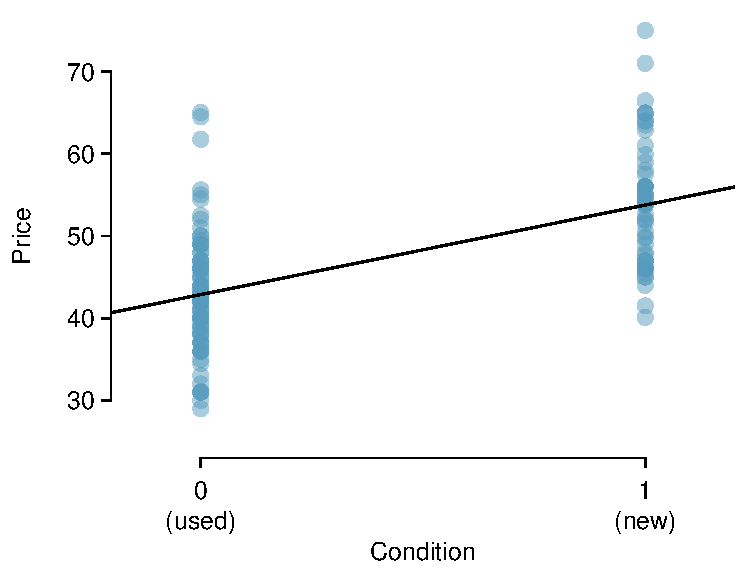
\includegraphics[width=0.5\textwidth]{figures/marioKartSingle/marioKartSingle}
	\end{figure}
\end{frame}
\begin{frame}{Adding more predictors}
	\textbf{Multiple regression}\\
	Include all the potentially important variables simultaneously.
	\begin{eqnarray*}
	\widehat{\text{price}}
		&=& \beta_0 + \beta_1\times \text{cond\_new} +
			\beta_2\times \text{stock\_ photo}  \\
		&\qquad&  + \beta_3 \times  \text{duration} +
			\beta_4 \times  \text{wheels} 
		\end{eqnarray*}
		\textbf{Or}
		\begin{eqnarray*}
	\hat{y} &=& \beta_0 + \beta_1 x_1 + \beta_2 x_2 +
			\beta_3 x_3 + \beta_4 x_4
		\end{eqnarray*}
		\end{frame}
		\begin{frame}{Fitting the model}
		Estimate the parameters $\beta_0$, $\beta_1$, ..., $\beta_4$.\\
		Process(similar to simple regression):
			\begin{itemize}
				\item Evaluate the sum squared residuals
				\[SSE=\sum e^2_i=\sum (y_i-\hat{y}_i)^2\]
				\item Select $b_0$, $b_1$, ..., $b_4$ that minimise SSE. 
			\end{itemize}
		\end{frame}
		\begin{frame}{Fitting the model}
			In practice we retrieve the following table.
			\begin{table}[ht]
			
					\resizebox{0.8\textwidth}{!}{
					\centering
			\begin{tabular}{rrrrr}
			  \hline
			  \vspace{-3.7mm} & & & & \\
			 & Estimate & Std. Error & t value & Pr($>$$|$t$|$) \\ 
			  \hline
			  \vspace{-3.8mm} & & & & \\
			(Intercept) & 36.2110 & 1.5140 & 23.92 & 0.0000 \\ 
			  cond\_\hspace{0.3mm}new & 5.1306 & 1.0511 & 4.88 & 0.0000 \\ 
			  stock\_\hspace{0.3mm}photo & 1.0803 & 1.0568 & 1.02 & 0.3085 \\ 
			  duration & -0.0268 & 0.1904 & -0.14 & 0.8882 \\ 
			  wheels & 7.2852 & 0.5547 & 13.13 & 0.0000 \\ 
			   \hline
			   &&&\multicolumn{2}{r}{$df=136$}
			\end{tabular}}
			
			\end{table}
			The multiple regression model is:
			\[\hat{y} = 36.21 + 5.13x_1 + 1.08x_2 - 0.027x_3 + 7.29x_4\]
		\end{frame}
		\begin{frame}{Interpretation of the parameters}
			\[\hat{y} = 36.21 + 5.13x_1 + 1.08x_2 - 0.027x_3 + 7.29x_4\]
			\small
			\begin{itemize}
				\item  The estimated coefficient of variable $x_4$ (Wii wheels) is $\beta_4= 7.29$. \\ This implies that the average difference in auction price for each additional Wii wheel included, \textbf{holding all the other variables constant}, is $7.29$.
				\item The estimated intercept is $36.21$, this is the model's predicted price when each of the variables take value zero. However, when the auction duration is 0, that implies that the auction has not started yet, so the price must be zero. Hence, the intercept does not provide any insight in this case.
				\end{itemize}
	\end{frame}
	\begin{frame}{Adjusted $R^2$}
		\small\begin{itemize}
			\item Simple linear regression
			\begin{eqnarray*}
			R^2& =& 1 - \frac{\text{variability in residuals}}{\text{variability in the outcome}}\\
				&=& 1 - \frac{Var(e)}{Var(y)}
			\end{eqnarray*}
			\item Adjusted $R^2$ for multiple regression
			\begin{eqnarray*}
			R_{adj}^{2} &=& 1-\frac{Var(e) / (n-k-1)}{Var(y) / (n-1)}\\
				&=& 1-\frac{Var(e)}{Var(y)} \times \frac{n-1}{n-k-1}
			\end{eqnarray*}
			where $n$ is the number of cases used to fit the model and $k$ is the number of predictor variables in the model.
		\end{itemize}
	\end{frame}
	\begin{frame}{Model Selection}
		\begin{itemize}
			\item A model that includes all available explanatory variables is often referred to as the \textbf{full model.}
			\item Is the full model the optimal model?
			\begin{itemize}
				\item Not necessarily. 
			\end{itemize}
			\item Explore different model selection strategies.
		\end{itemize}
	\end{frame}
	\begin{frame}{Mario Kart (again!)}
		\begin{table}[ht]
				\resizebox{0.7\textwidth}{!}{
				\centering
		\begin{tabular}{rrrrr}
		  \hline
		  \vspace{-3.7mm} & & & & \\
		 & Estimate & Std. Error & t value & Pr($>$$|$t$|$) \\ 
		  \hline
		  \vspace{-3.8mm} & & & & \\
		(Intercept) & 36.2110 & 1.5140 & 23.92 & 0.0000 \\ 
		  cond\_\hspace{0.3mm}new & 5.1306 & 1.0511 & 4.88 & 0.0000 \\ 
		  stock\_\hspace{0.3mm}photo & 1.0803 & 1.0568 & 1.02 & 0.3085 \\ 
		  duration & -0.0268 & 0.1904 & -0.14 & 0.8882 \\ 
		  wheels & 7.2852 & 0.5547 & 13.13 & 0.0000 \\ 
		   \hline
		  \vspace{-3.6mm} & & & & \\
		\multicolumn{3}{l}{$R_{adj}^2 = 0.7108$}&\multicolumn{2}{r}{$df=136$}
		\end{tabular}}
		\end{table}
	\small	The last column of the table lists p-values that can be used to assess hypotheses of the following form:
		\begin{itemize}
		\setlength{\itemsep}{0mm}
		\item[$H_0$:] $\beta_i = 0$ when the other explanatory variables are included in the model.
		\item[$H_A$:] $\beta_i \neq 0$ when the other explanatory variables are included in the model.
		\end{itemize}
	\end{frame}
	\begin{frame}{Selecting predictors}
		
			\begin{table}[ht]
					\resizebox{0.7\textwidth}{!}{
					\centering
			\begin{tabular}{rrrrr}
			  \hline
			  \vspace{-3.7mm} & & & & \\
			 & Estimate & Std. Error & t value & Pr($>$$|$t$|$) \\ 
			  \hline
			  \vspace{-3.8mm} & & & & \\
			(Intercept) & 36.2110 & 1.5140 & 23.92 & 0.0000 \\ 
			  cond\_\hspace{0.3mm}new & 5.1306 & 1.0511 & 4.88 & 0.0000 \\ 
			  stock\_\hspace{0.3mm}photo & 1.0803 & 1.0568 & 1.02 & 0.3085 \\ 
			  duration & -0.0268 & 0.1904 & -0.14 & 0.8882 \\ 
			  wheels & 7.2852 & 0.5547 & 13.13 & 0.0000 \\ 
			   \hline
			  \vspace{-3.6mm} & & & & \\
			\multicolumn{3}{l}{$R_{adj}^2 = 0.7108$}&\multicolumn{2}{r}{$df=136$}
			\end{tabular}}
			\end{table}
			\textbf{Identify}  the variables in the model that may not be helpful.
		\end{frame}
		\begin{frame}{Selecting predictors}
			\begin{itemize}
				\item The $p-$value for the auction duration is $0.8882$, which indicates that there is not statistically significant evidence that the duration is related to the total auction price when accounting for the other variables.
				\item The $p-$value for the  condition of the game is zero, which indicates there is strong evidence that a game's condition (new or used) has a real relationship with the total auction price, when accounting for the other variables..
			\end{itemize}
		\end{frame}
		\begin{frame}{Two model selection strategies}
			\textbf{Stepwise} model selection strategies
			\begin{itemize}
				\item Backward selection
				\item Forward selection
			\end{itemize}
		\end{frame}
		\begin{frame}{Model selection strategy}
			\textbf{Backward elimination strategy}
			\begin{itemize}
				\item Start from a \textbf{full} model
				\item Drop the variable with the largest $p-$value
				\item Refit the model
				\item Drop the variable with the largest $p-$value
				\item Refit the model\dots
			\end{itemize}
			\textbf{Repeat} until happy...\\
			\textbf{Note:} In the case, two variables have the same $p-$value examine the adjusted $R^2.$
		\end{frame}
		\begin{frame}{Backward selection on Mario}
			\small
			The multiple regression model is:
			\[\hat{y} = 36.21 + 5.13x_1 + 1.08x_2 - 0.027x_3 + 7.29x_4\]
			with 
			\begin{table}[ht]
			
					\resizebox{0.7\textwidth}{!}{
					\centering
			\begin{tabular}{rrrrr}
			  \hline
			  \vspace{-3.7mm} & & & & \\
			 & Estimate & Std. Error & t value & Pr($>$$|$t$|$) \\ 
			  \hline
			  \vspace{-3.8mm} & & & & \\
			(Intercept) & 36.2110 & 1.5140 & 23.92 & 0.0000 \\ 
			  cond\_\hspace{0.3mm}new & 5.1306 & 1.0511 & 4.88 & 0.0000 \\ 
			  stock\_\hspace{0.3mm}photo & 1.0803 & 1.0568 & 1.02 & 0.3085 \\ 
			  duration & -0.0268 & 0.1904 & -0.14 & 0.8882 \\ 
			  wheels & 7.2852 & 0.5547 & 13.13 & 0.0000 \\ 
			   \hline
			  \multicolumn{3}{l}{$R_{adj}^2 = 0.7108$}&\multicolumn{2}{r}{$df=136$}
			\end{tabular}}
			
			\end{table}
Which variable should we eliminate?			
		\end{frame}
		\begin{frame}{Backwards selection on Mario}
			After eliminating the \textbf{duration} variable, we refit the model:
			\begin{table}[ht]
					\resizebox{0.9\textwidth}{!}{
					\centering
			\begin{tabular}{rrrrr}
			  \hline
			  \vspace{-3.7mm} & & & & \\
			 & Estimate & Std. Error & t value & Pr($>$$|$t$|$) \\ 
			  \hline
			  \vspace{-3.8mm} & & & & \\
			(Intercept) & 36.0483 & 0.9745 & 36.99 & 0.0000 \\ 
			  cond\_\hspace{0.3mm}new & 5.1763 & 0.9961 & 5.20 & 0.0000 \\ 
			  stock\_\hspace{0.3mm}photo & 1.1177 & 1.0192 & 1.10 & 0.2747 \\ 
			  wheels & 7.2984 & 0.5448 & 13.40 & 0.0000 \\ 
			   \hline
			  \vspace{-3.6mm} & & & & \\
			\multicolumn{3}{l}{$R_{adj}^2 = 0.7128$}&&\small$df=137$
			\end{tabular}}
			\end{table}
			Which variable should we eliminate?	
		\end{frame}
			\begin{frame}{Backwards selection on Mario}
				After eliminating the \textbf{stock photo} variable, we refit the model:
				\begin{table}[ht]
						\resizebox{0.9\textwidth}{!}{
						\centering
				\begin{tabular}{rrrrr}
				  \hline
				  \vspace{-3.7mm} & & & & \\
				 & Estimate & Std. Error & t value & Pr($>$$|$t$|$) \\ 
				  \hline
				  \vspace{-3.8mm} & & & & \\
				(Intercept) & 36.7849 & 0.7066 & 52.06 & 0.0000 \\ 
				  cond\_\hspace{0.3mm}new & 5.5848 & 0.9245 & 6.04 & 0.0000 \\ 
				  wheels & 7.2328 & 0.5419 & 13.35 & 0.0000 \\ 
				   \hline
				  \vspace{-3.6mm} & & & & \\
				\multicolumn{3}{l}{$R_{adj}^2 = 0.7124$}&&\small$df=138$
				\end{tabular}}
				\end{table}
				Since all the $p-$values are equal to zero, we conclude that this is the optimal model given the variables.
			\end{frame}
			\begin{frame}{Model selection strategy}
				\textbf{Forward elimination strategy}
				\begin{itemize}
					\item Start from a  model that includes no variables
					\item Fit each of the possible models with just one variable.
					\item Select the variable with the smallest $p-$values.
					\item Add the variable to the model
					\item Expand this model by adding one of the remaining variables.
					\item Fit the respective models
					\item Select the variable with the smallest $p-$values.
					\item Add the variable to the model\dots
				\end{itemize}
				\textbf{Repeat} until happy...\\
				\textbf{Note:} In the case, two variables have the same $p-$value examine the adjusted $R^2.$
			\end{frame}
			\begin{frame}{Summary}
				\begin{itemize}
					\item The \textbf{backward-elimination} strategy begins with the largest model and eliminates variables one-by-one until we are satisfied that all remaining variables are important to the model. 
					
\item The \textbf{forward-selection} strategy starts with no variables included in the model, then it adds in variables according to their importance until no other important variables are found.
\end{itemize}
			\end{frame}
			\begin{frame}{Model assumptions}
				\begin{center}
			\textbf{Are the model's assumptions satisfied?}
			\end{center}
			\end{frame}
			\begin{frame}{Assumptions}
				
				\textbf{Multiple regression} methods using the model
				\begin{align*}
				\hat{y} &= \beta_0 + \beta_1x_1 + \beta_2x_2 + \cdots + \beta_kx_k
				\end{align*}
				generally depend on the following four \textbf{assumptions}:
				\begin{enumerate}
				\setlength{\itemsep}{0mm}
				\item the residuals of the model are nearly normal,
				\item the variability of the residuals is nearly constant,
				\item the residuals are independent, and
				\item each variable is linearly related to the outcome.
				\end{enumerate}
			\end{frame}
			\begin{frame}{Nearly normal residuals}
				\textbf{Normal probability plot for the residuals}
				\begin{figure}
				\centering
	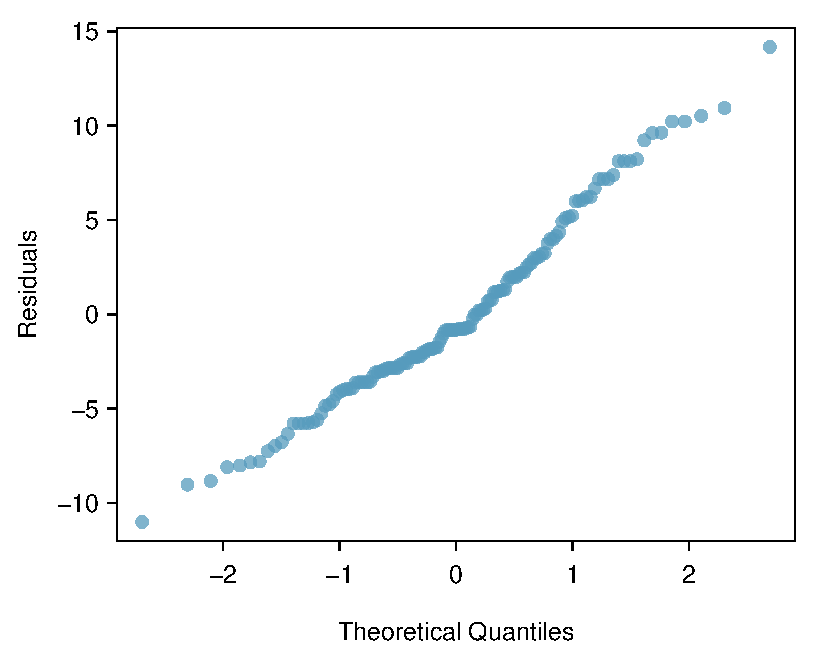
\includegraphics[width=0.71\textwidth]{figures/marioKartDiagnostics/mkDiagnosticNormalQuantilePlot}
				\end{figure}
			\end{frame}
			\begin{frame}{Near constant variability}
				\textbf{Absolute values of residuals against fitted values}
				\begin{figure}
				\centering
				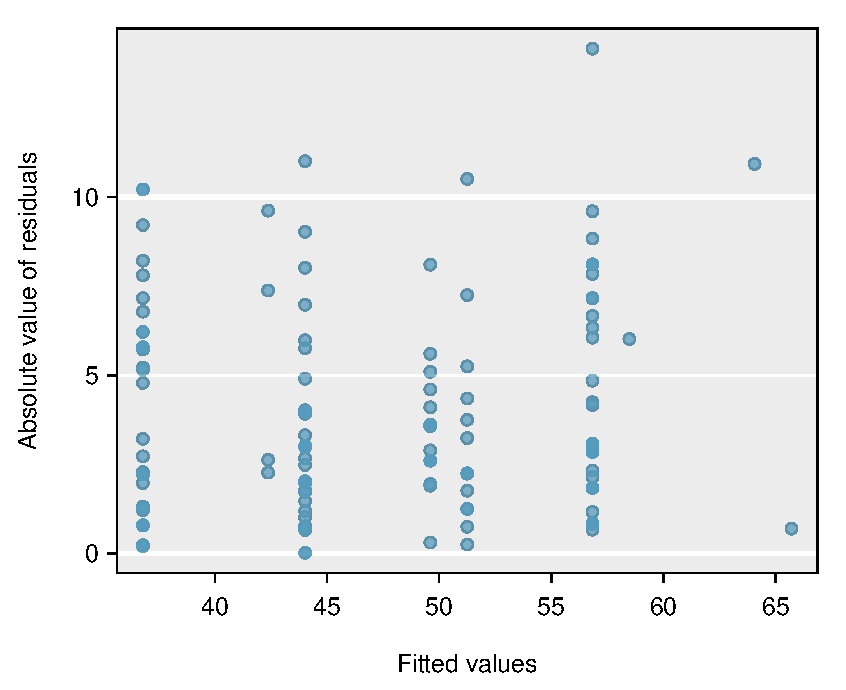
\includegraphics[width=0.72\textwidth]{figures/marioKartDiagnostics/mkDiagnosticEvsAbsF}
			
				\label{mkDiagnosticEvsAbsF}
				\end{figure}
			\end{frame}
			\begin{frame}{Residuals are independent}
				\textbf{Residuals in order of their data collection}
				\begin{figure}
				\centering
				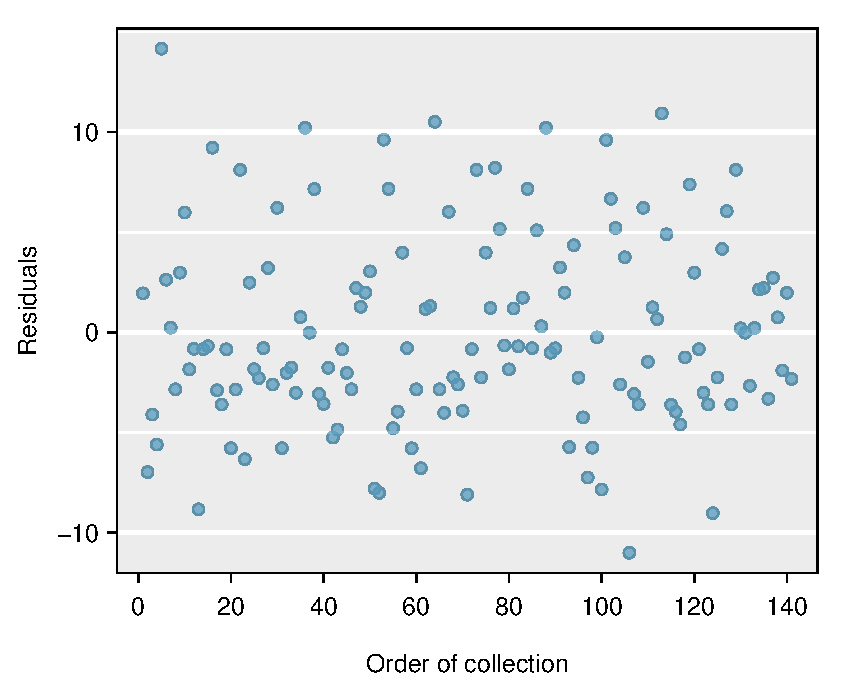
\includegraphics[width=0.72\textwidth]{figures/marioKartDiagnostics/mkDiagnosticInOrder}
				\end{figure}
			\end{frame}
			\begin{frame}{Each variable is linearly related to the outcome}
				\textbf{Residuals against each predictor variable}
				\begin{figure}
				\centering
				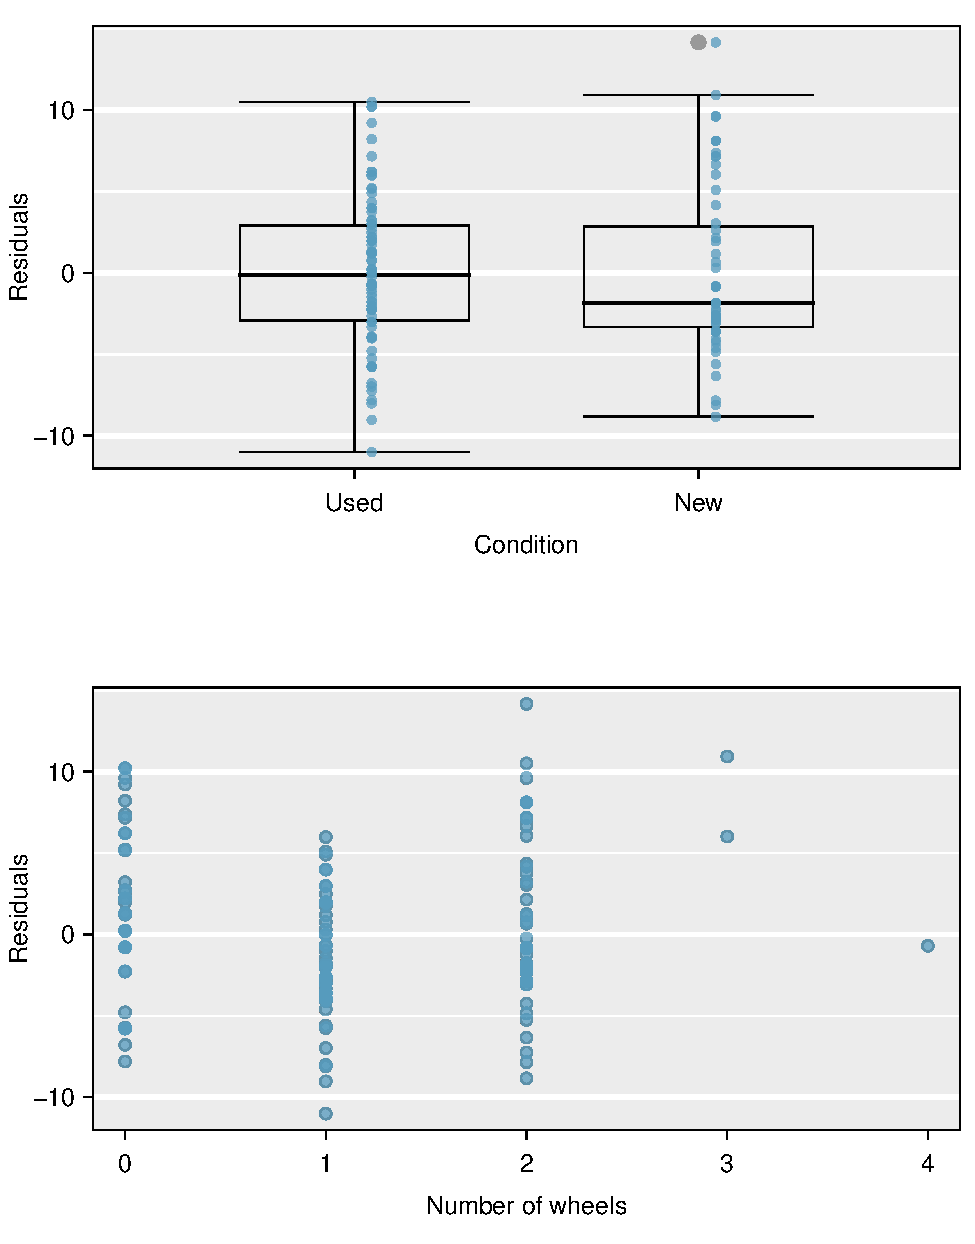
\includegraphics[width=0.5\textwidth]{figures/marioKartDiagnostics/mkDiagnosticEvsVariables}
				\end{figure}
				We should not see any trend in the residual plots.
			\end{frame}
			\begin{frame}{Notes}
				\textbf{Matrix representation of data}\\
				Multi-regression model:
				\[y=\beta_0+\beta_1x_1+\dots+\beta_kx_k+\epsilon\]
				 If we have $n$ observations then,
				\[y_i=\beta_0+\beta_1x_{i1}+\dots+\beta_kx_{ik}+\epsilon_i,\]
				where $x_{ij}$ is the value of the $jth$ independent variable in the $ith$ observation, $j=1,\dots,n.$
			\end{frame}
			\begin{frame}{Notes}
				\textbf{Matrix notation}
			\small	\begin{eqnarray*}
				Y=	\left[\begin{array}{c} y_1\\
					y_2\\
					\vdots\\
					y_n
				\end{array}\right] &{}& 	X=	\left[\begin{array}{ccccc} 1 & x_{11} &x_{12}&\dots&x_{1k}\\
						 1 & x_{11} &x_{12}&\dots&x_{1k}\\
						\vdots\\
					 1 & x_{n1} &x_{n2}&\dots&x_{nk}
					\end{array}\right]\\
					\beta=\left[\begin{array}{c} \beta_0\\
						\beta_1\\
						\vdots\\
						\beta_k
					\end{array}\right] &{}& 	\epsilon=\left[\begin{array}{c} \epsilon_1\\
							\epsilon_2\\
							\vdots\\
							\epsilon_n
						\end{array}\right] 
				\end{eqnarray*}
			Hence, the matrix representation of the multi-regression model is
			\[Y=X\beta+\epsilon\]	
			
			\end{frame}
			\begin{frame}{Notes}
				\textbf{Transformation of categorical variables}
			\small	\begin{itemize}
					\item\textbf{Two levels} categorical variable, ex. F/M, Yes/No, can be represented as
				\small	\[x=\left\{\begin{array}{lr} 0,& \text{ if F}\\
					1, &\text{ if M}\end{array}\right.\]
					\item \textbf{k-levels} categorical variable, ex. agree, disagree, na.
					\\ Introduce $k-1$ dummy variables
					\[x_1=\left\{\begin{array}{lr} 1,& \text{ if agree }\\
					0, &\text{ otherwise}\end{array}\right. x_2=\left\{\begin{array}{lr} 1,& \text{ if disagree}\\
					0, &\text{otherwise}\end{array}\right.\]
					\item $\begin{array}{ccc}
					& x_1 & x_2\\
					\text{agree}& 1 & 0\\
					\text{disagree}&0&1\\
					\text{na}&0&0 
					\end{array}$
				\end{itemize}

			\end{frame}
			\begin{frame}{Logistic regression}
				For $y$  a \textbf{numerical response} variable and $k$ predictors, $x_1,x_2,\dots,x_k,$ our goal is to find a relation between them:
				\[y=f(x_1,x_2,\dots,x_k)\]
				\begin{itemize}
					\item  For a \textbf{numerical  variable} $y$, we can try a \textbf{multi-regression} model:
				\[\hat{y} = \beta_0 + \beta_1 x_1 + \beta_2 x_2 + \cdots + \beta_k x_k \]
	\item What about a \textbf{categorical variable} $y$?
			\end{itemize}
				\end{frame}
				\begin{frame}{Spam again...}
					\begin{table}[!htbp] \centering 
						\resizebox{0.97\textwidth}{!}{
					\begin{tabular}{@{\extracolsep{5pt}} cccccccccccc} 
					\\[-1.8ex]\hline 
					\hline \\[-1.8ex] 
					 & spam & to\_multiple & cc & attach & dollar & winner & inherit & password & format & re\_subj & exclaim\_subj \\ 
					\hline \\[-1.8ex] 
					1 & $0$ & $0$ & $0$ & $0$ & $0$ & $0$ & $0$ & $0$ & $1$ & $1$ & $0$ \\ 
					2 & $0$ & $0$ & $0$ & $0$ & $0$ & $0$ & $0$ & $0$ & $1$ & $0$ & $0$ \\ 
					3 & $1$ & $0$ & $1$ & $1$ & $0$ & $0$ & $0$ & $0$ & $0$ & $0$ & $0$ \\ 
					4 & $0$ & $0$ & $0$ & $0$ & $0$ & $0$ & $0$ & $0$ & $0$ & $0$ & $0$ \\ 
					5 & $0$ & $0$ & $0$ & $0$ & $1$ & $0$ & $0$ & $1$ & $1$ & $0$ & $0$ \\ 
					6 & $0$ & $0$ & $0$ & $0$ & $0$ & $0$ & $0$ & $0$ & $0$ & $0$ & $0$ \\ 
					\hline \\[-1.8ex] 
				\end{tabular} }
					\end{table}
					\begin{table}
						\resizebox{0.6\textwidth}{!}{
					\begin{tabular}{lp{10.5cm}}
					\hline
					{\bf variable} & {\bf description} \\
					\hline
					spam & Specifies whether the message was spam. \\
					to\_multiple & An indicator variable for if more than one person was listed in the \emph{To} field of the email.  \\
					cc & An indicator for if someone was CCed on the email. \\
					attach & An indicator for if there was an attachment, such as a document or image.   \\
					dollar & An indicator for if the word ``dollar'' or dollar symbol (\$) appeared in the email.  \\
					winner & An indicator for if the word ``winner'' appeared in the email message.  \\
				inherit & An indicator for if the word ``inherit'' (or a variation, like ``inheritance'') appeared in the email.  \\
					password & An indicator for if the word ``password'' was present in the email.  \\
					format & Indicates if the email contained special formatting, such as bolding, tables, or links    \\
					re\_subj & Indicates whether ``Re:'' was included at the start of the email subject.   \\
					exclaim\_subj & Indicates whether any exclamation point was included in the email subject.    \\
					\hline
					\end{tabular}}
					\end{table}
				\end{frame}
				\begin{frame}{Logistic regression}
				\textbf{Explanatory variable:}\\
				  multiple recipients, cc, dollar, winner: $0$\\
				inherit, password, format, re\_subj, exclaim\_subj:$1$\\
				\textbf{Response variable:}\\
				Spam:0 \textbf{or} 1?\\
				\textbf{Logistic regression:} The probability that the email is spam, given this explanatory variables.
					\end{frame}
					\begin{frame}{Logistic regression}
					\begin{itemize}
						\item $y:$ \textbf{categorical response variable }, with two levels $\{0,1\}$
						\item  $x_1,x_2,\dots,x_k:$ $k$  \textbf{predictors.} 
					\end{itemize}
						Then model for \textbf{logistic regression} is
						\[p=\frac{1}{1+e^{-(\beta_0+\beta_1x_1+\dots+\beta_kx_k)}},\] 
 where $p$ is the probability of $y=1$.
					\end{frame}
					\begin{frame}{Logistic function}
						\textbf{Logistic/Sigmoid} function
						\begin{figure}
						\centering
						\begin{minipage}{0.8\textwidth}
						  \centering
						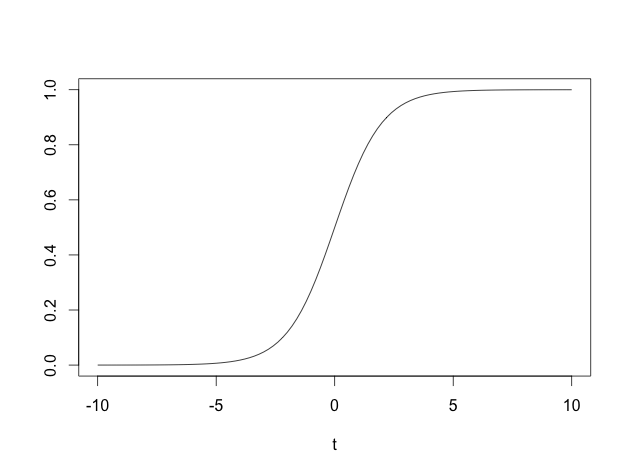
\includegraphics[width=0.8\textwidth]{figures/sigmoid}
					\end{minipage}%
					\begin{minipage}{0.2\textwidth}
						\small$f(t)=\frac{1}{1+e^{-t}}$
					\end{minipage}
						\end{figure}
						\end{frame}
						\begin{frame}{Logistic regression}
						\textbf{ Likelihood function}
						
	\small					\begin{eqnarray*}
						&&L(y_1,\dots,y_n;x_1,\dots,x_k,\beta_0,\dots,\beta_k)=\\&{}&\Pi^n_{i=1}p(x_{i1},\dots,x_{ik})^{y_i}(1-p(x_{i1},\dots,x_{in}))^{1-y_i},
						\end{eqnarray*}
		where $p(x_{i1},\dots,x_{in})=\frac{1}{1+e^{-(\beta_0+\beta_1x_{i1}+\dots+\beta_kx_{ik})}}.$\\
		\vspace{0.3cm}
		The parameters for the logistic regression are the \textbf{maximum likelihood estimator}; $\beta_0,\dots,\beta_k$ that maximise $L(y_1,\dots,y_n;x_1,\dots,x_k,\beta_0,\dots,\beta_k).$
						\end{frame}
						\begin{frame}{Logistic regression}
							\textbf{Logistic model} for single predictor to\_multiple.
							\[p=\frac{1}{1+e^{2.12+1.81x}}\]
							If an email has no multiple recipients, to probability of it being spam is
							\[p=\frac{1}{1+e^{2.12}}=0.11,\]
							else the probability is
							\[p=\frac{1}{1+e^{2.12+1.81x}}=0.02\]
						\end{frame}
						\begin{frame}{Logistic regression}
							\textbf{Logistic regression model} for $11$ predictors:
							\begin{table}[ht]
								\centering
								\resizebox{0.7\textwidth}{!}{
							\begin{tabular}{rrrrr}
							  \hline
							  \vspace{-3.7mm} & & & & \\
							 & Estimate & Std. Error & z value & Pr($>$$|$z$|$) \\ 
							  \hline
							  \vspace{-3.8mm} & & & & \\
							(Intercept) & -0.8362 & 0.0962 & -8.69 & 0.0000 \\ 
							  to\_\hspace{0.3mm}multiple & -2.8836 & 0.3121 & -9.24 & 0.0000 \\ 
							  winner & 1.7038 & 0.3254 & 5.24 & 0.0000 \\ 
							  format & -1.5902 & 0.1239 & -12.84 & 0.0000 \\ 
							  re\_\hspace{0.3mm}subj & -2.9082 & 0.3708 & -7.84 & 0.0000 \\ 
							  exclaim\_\hspace{0.3mm}subj & 0.1355 & 0.2268 & 0.60 & 0.5503 \\ 
							  cc & -0.4863 & 0.3054 & -1.59 & 0.1113 \\ 
							  attach & 0.9790 & 0.2170 & 4.51 & 0.0000 \\ 
							  dollar & -0.0582 & 0.1589 & -0.37 & 0.7144 \\ 
							  inherit & 0.2093 & 0.3197 & 0.65 & 0.5127 \\ 
							  password & -1.4929 & 0.5295 & -2.82 & 0.0048 \\ 
							\hline
							\end{tabular}}
							\end{table}
						\end{frame}
						\begin{frame}{Logistic regression}
							After variable selection.
							\begin{table}[ht]
							\centering
							\resizebox{0.7\textwidth}{!}{
							\begin{tabular}{rrrrr}
							  \hline
							  \vspace{-3.7mm} & & & & \\
							 & Estimate & Std. Error & z value & Pr($>$$|$z$|$) \\ 
							  \hline
							  \vspace{-3.8mm} & & & & \\
							(Intercept) & -0.8595 & 0.0910 & -9.44 & 0.0000 \\ 
							  to\_\hspace{0.3mm}multiple & -2.8372 & 0.3092 & -9.18 & 0.0000 \\ 
							  winner & 1.7370 & 0.3218 & 5.40 & 0.0000 \\ 
							  format & -1.5569 & 0.1207 & -12.90 & 0.0000 \\ 
							  re\_\hspace{0.3mm}subj & -3.0482 & 0.3630 & -8.40 & 0.0000 \\ 
							  attach & 0.8643 & 0.2042 & 4.23 & 0.0000 \\ 
							  password & -1.4871 & 0.5290 & -2.81 & 0.0049 \\ 
							\hline
							\end{tabular}}
							\end{table}
						\end{frame}
						\begin{frame}{Logistic regression}
		\small					\[p=\frac{1}{1+e^{-0.859-2.837x_1+1.737x_2-1.557x_3-3.05x_4+0.854x_5-1.487x_6}}\]
		
						\end{frame}
\end{document}